% providecommand redefines the command only if not already defined.
% This is useful to define a different path to other files for subfiles compared to the main thesis.
\providecommand{\main}{..} % Relative path of the main thesis (`..` represents the parent directory)
\providecommand{\figures}{\main/figures}

% The subfiles document class uses the preamble from the file in the optional argument. Don't repeat it.
\documentclass[\main/ExampleThesis]{subfiles}

\begin{document}

\chapter{Introduction}
\label{ch:introduction}

\lipsum[1]%
\footnote{This is simply the ubiquitous ``Lorem Ipsum'' placeholder text for typesetting. This is a long footnote, and extends to more than just a single line.}

\section{\lipsum[150][1-3]}

\lipsum[2]

\begin{figure}[tbp]
  \centering
  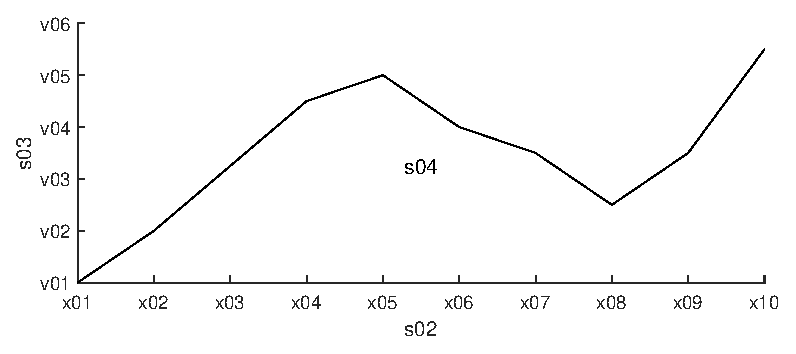
\includegraphics[width=.7\textwidth]{\figures/pictures/placeholder}
  \caption{The caption of the figure}
  \label{fig:placeholder1}
\end{figure}

\begin{figure}[tbp]
  \centering
  \includeplot[width=.8\textwidth]{\figures/plots/placeholder}
  \caption{The caption of the plot which is much longer than the other captions, since it should flow to the next line.}
  \label{fig:placeholder2}
\end{figure}

\begin{figure}[tbp]
  \centering
  \includediagram{\figures/diagrams/placeholder}
  \caption{The caption of the diagram. This diagram was created with Ti\emph{k}Z.}
  \label{fig:placeholder3}
\end{figure}

\section{\lipsum[150][4]}

\subsection{\lipsum[150][8]}

\lipsum[3]


 \cite{einstein, latexcompanion, knuthwebsite}

\end{document}